\Section{Splay и корневая оптимизация}{24 апреля}{Сергей Копелиович}

% \Subsection{Rope}

% \begin{Def}Rope -- интерфейс структуры данных, требующий, чтобы она умела производить с массивом следующие операции:
% \begin{InnerMyList}
% 	\item \t{insert(i)}, \t{erase(i)}
% 	\item \t{split(i)}, \t{merge(a, b)}, \t{rotate(k)}
% \end{InnerMyList}
% \end{Def}

% \up
% Обычно подразумевают, что структура все выше перечисленные операции умеет делать быстро, например, за $\O(\log n)$.
% Всё выше перечисленное умеют сбалансированные деревья по неявному ключу со \t{split} и \t{merge}.
% У нас уже есть AVL-tree, RB-tree, Treap, сегодня ещё появится Splay-tree.
% Кроме того есть структуры, в основе которых лежат не деревья поиска, удовлетворяющие интерфейсу Rope.
% Из таких у нас сегодня появятся Skip-List и SQRT-decomposition.

% \Subsection{Skip-list}

% Структура данных {\it односвязный список} хороша тем, что \t{split}, \t{merge}, \t{insert}, \t{erase}
% работают за $\O(1)$. За $\O(n)$ работает только операция поиска. Например \t{split(i) = find(i) + $\O(1)$}.
% Чтобы ускорить поиск можно добавить ссылки вперёд на $2^k$ шагов.

% \down
% \TODO: картинка с иллюстрацией структуры данных и нового \t{find}.
% \down

% Правда после \t{insert} и \t{erase} такие ссылки неудобно пересчитывать.\\
% Поэтому авторы Skip-List поступили хитрее.
% Skip-List -- $\log_2n$ списков. Нижний (нулевой) список -- все данные нам элементы.
% Каждый элемент из $i$-го списка с вероятностью $0.5$ содержится в $(i{+}1)$-м списке.
% Итого любой элемент в $i$-м списке содержится с вероятностью $2^{-i} \SO$\\
% $E[|List_i|] = n2^{-i} \SO$ суммарный размер всех списков $2n$.

% \begin{code}
% struct Node {
% 	Node *down, *right;
% 	int x, right_len;	
% };
% const int LOG_N = 17;
% vector<Node*> head[LOG_N+1]; // `для удобства считаем, что $\log n$ не меняется`
% Node* find( int i ) {
% 	Node *res;
% 	int pos = -1; // `в каждом списке голова -- фиктивный $(-1)$-й элемент`
% 	for (Node *v = head[LOG_N]; v; res = v, v = v->down)
% 		while (v->right && pos + v->right_len < i)
% 			pos += v->`\red{right\_len}`, v = v->right;
% 	return res; // `максимальный ключ меньший $x$ в нижнем списке`
% }
% \end{code}

% \begin{Lm}Матожидание времени работы \t{find} -- $\O(\log n)$.\end{Lm}
% \begin{proof}
% 	На каждом шаге \t{for} матожидание число шагов $\O(1)$.
% \end{proof}

% Чтобы удалить $i$-элемент, сделаем \t{find(i)}, который в каждом списке пройдёт по элементу, предшествующему $i$.
% Для каждого списка: если $i$ был в списке, удалим за $\O(1)$, сложим длины соседних рёбер. Если $i$ не было, уменьшим длину ссылки вправо на $1$.

\Subsection{Splay tree}

Splay-дерево --- самобалансирующееся BST, не хранящее в вершине никакой дополнительной информации.
В худшем случае глубина может быть линейна, но амортизированное время всех операций получится $\O(\log n)$.
Возьмём обычное не сбалансированное дерево. При \t{add}/\t{del}.\\
Модифицируем \t{add}: спустившись вниз до вершины $v$ он самортизирует потраченное время вызовом \t{Splay(v)},
которая последовательными вращениями протолкнёт $v$ до корня.

\THE{Zig-zig вращение}

\vspace*{-2em}
\begin{center}
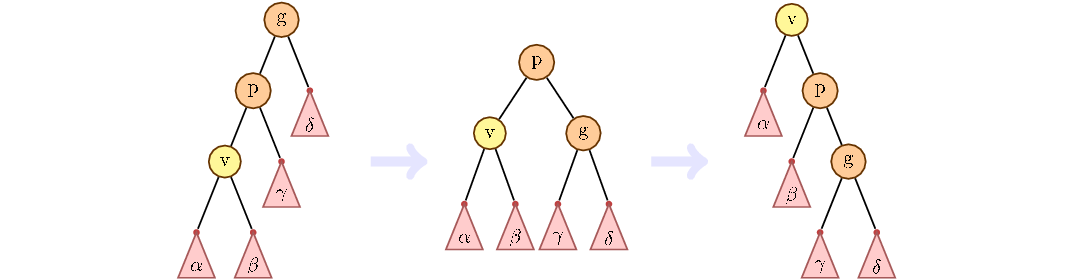
\includegraphics{pics/zig-zig.png}
\end{center}

\THE{Zig-zag вращение}

\vspace*{-2em}
\begin{center}
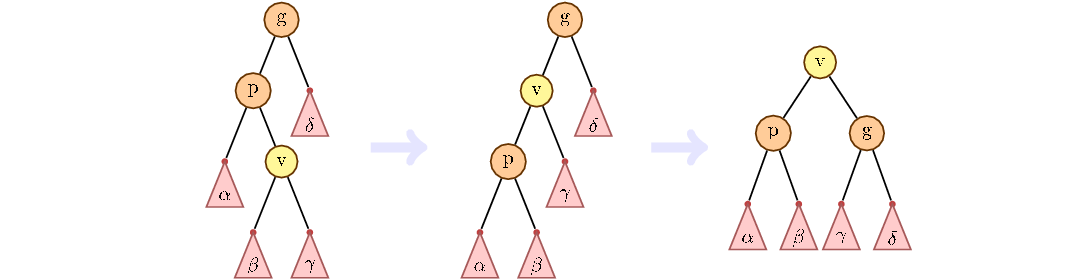
\includegraphics{pics/zig-zag.png}
\end{center}

\THE{Если дедушки нет,} сделаем обычный single rotation (zig).

\vspace*{-2em}
\begin{center}
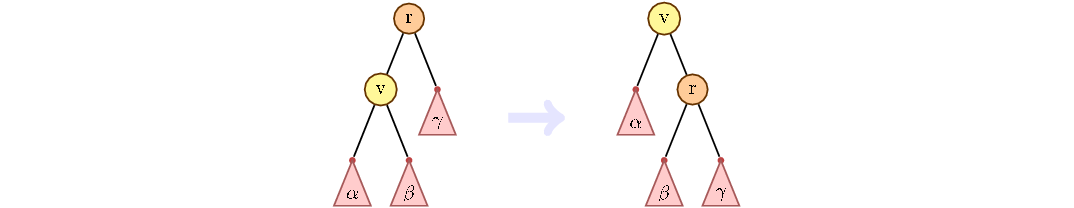
\includegraphics{pics/single-rotate.png}
\end{center}

В частности из картинок видно, что все вращения выражаются через single rotation.

\pagebreak

Любые другие операции со splay деревом делаются также, как и \t{add}: пусть $v$ -- самая глубокая вершина, до которой мы спустились 
$\SO$ вызовем \t{splay(v)}, который протолкнёт $v$ в корень и самортизирует время работы.
При этом всегда время \t{splay(v)} не меньше остальной полезной части $\SO$
осталось оценить время работы \t{splay}.

\begin{Lm}$x, y > 0, x + y = 1 \SO \log x + \log y \le -2$\end{Lm}
\begin{proof}$\log x + \log y = \log x + \log (1-x) = \log x(1-x) \le \log\mfrac{1}{2} \cdot\red{2} = -2$\end{proof}
\begin{Lm}$x, y > 0, x + y = C \SO \log x + \log y \le 2\log C - 2$\end{Lm}
\begin{proof}$\log x + \log y = 2\log C + \log\mfrac{x}{C} + \log\mfrac{y}{C} \le 2\log C - 2$\end{proof}

Теперь введём потенциал. Ранг вершины $R_v = \log(size_v)$, где $size_v$ -- размер поддерева.
Потенциал $\PHI = \sum R_v$. Заметим сразу, что для пустого дерева $\PHI_0 = 0$ и $\forall$ момент времени $\PHI \ge 0$.
Оценим амортизированное время операции \t{splay}, поднявшей $v$ в $u$:

\begin{Thm}\label{thm@splay}
$\forall v, u \ a_{v\to u} \le 3(R_u - R_v) + 1 = 3\log\mfrac{size_u}{size_v} + 1$\end{Thm}
\begin{proof}
Полное доказательство доступно \href{http://www.cs.cornell.edu/courses/cs3110/2011sp/recitations/rec25-splay/splay.htm}{здесь}.
Мы разберём только случай zig-zig. Оставшиеся два аналогичны. ${+}1$ вылезет из случая zig (отсутствие деда).
Итак, $a = t + \Delta \PHI = $\\
$2 + (R_{x'}+R_{y'}+R_{z'}) - (R_x + R_y + R_z) = 2 + R_{y'} + R_{z'} - R_x - R_y \le 2 + R_{x'} + R_{z'} - 2R_x = F$.
\begin{verbatim}
      z             x' 
     / \           / \
    y   D         A   y'
   / \      -->      / \    	            (A < x < B < y < C < z < D)
  x   C             B   z'
 / \                   / \
A   B                 C   D
\end{verbatim}
Мы хотим показать $F \le 3(R_{x'} - R_x) \EQ R_{z'} \le 2R_{x'} - R_x - 2 \EQ R_{z'} + R_x \le 2R_{x'} - 2$.\\
Теперь вспомним, что $R_{z'} = \log(C+D+1), R_x = \log(A+B+1) \overset{\text{лемма}}{\SO} $\\
$R_{z'} + R_{x} \le 2\log(A+B+C+D+2)-2 \le 2R_{x'} - 2$.
\end{proof}

\begin{Cons}Среднее время одной операции в splay-дереве -- $\O(\log n)$.\end{Cons}
\begin{proof}
$\PHI_0 = 0, \PHI \ge 0 \SO \mfrac{1}{m}\sum t_i \le a_i = \O(\log n)$.
\end{proof}

\begin{Rem}В теорему вместо $size_v$ можно подставить любой взвешенный размер: \\
$size_v = w_v + size_l + size_r$, где $w_v$ -- вес вершины. \\
Чтобы потенциал всегда был неотрицательный, потребуем $w_v \ge 1 \SO \log w_v \ge 0$.\end{Rem}

Теперь о преимуществах splay-дерева. Элемент, к которому мы обращаемся чаще, оказывается ближе к корню, поэтому обращения к нему быстрее.
Формально это можно записать так:

\begin{Thm}Пусть к splay-дереву поступают только запросы \t{find(v)}, $k_v$ -- количество обращений
к вершине $v$, $m = \sum k_v$. Тогда суммарное время всех \t{find} равно $\sum_v k_v (3\log\mfrac{n{+}m}{k_v} + 1)$.
\end{Thm}

\vspace*{-1.0em}
\begin{proof}
Внутри суммы $k_v$ -- количество запросов к $v$, $(3\log\mfrac{\red{n{+}m}}{k_v} + 1)$ -- время на один запрос.
Эта оценка на время получается из \autoref{thm@splay} подстановкой веса вершины $w_v = \max(k_v\red{, 1)}$.\\
Тогда $size_{root} \le n{+}m$ и время $splay(v) \le 3\log\mfrac{size_{root}}{size_v} + 1 \le 3\log\mfrac{size_{root}}{k_v} + 1$.
\end{proof}

На \href{http://acm.math.spbu.ru/~sk1/courses/1617s_au/practice/170504.pdf}{практике} 
мы также доказали теорему о времени работы бора (задача 11, есть разбор).

\down
В той ж практике в 9-й задаче предлагается более быстрая \t{top-down} реализация splay-дерева.

\down
\Subsection{SQRT decomposition}

\up
\Subsubsection{Корневая по массиву}

{\it Идея:} разобьём массив на $\sqrt{n}$ частей (кусков) размера $k=\sqrt{n}$.

\THE{Сумма на отрезке и изменение в точке}

Решение: $\O(1)$ на изменение, $\O(\sqrt{n})$ на запрос суммы.
$\forall i$ для $i$ куска поддерживаем сумму~\t{s[i]}.
\begin{code}
void change(i, x):
	s[i/k] += (x-a[i]), a[i]=x
int get(l, r): // [l, r)
	int res = 0
	while (l < r && l % k != 0) res += a[l++]; // `левый хвост`
	while (l < r && r % k != 0) res += a[--r]; // `правый хвост`
	return accumulate(s + l / k, s + r / k, res); // `цельные куски`
\end{code}
Запрос на отрезке разбивается на два хвоста длины $\sqrt{n}$ и не более $\sqrt{n}$ цельных кусков.

\down
Решение за $\O(\sqrt{n})$ на изменение и $\O(1)$ на запрос суммы:
будем поддерживать частичные суммы для каждого куска и для массива $s$.
При изменении пересчитаем за $\O(\sqrt{n})$ частичные суммы внутри куска номер \t{i/k}
и частичные суммы массива $s$. Суммы на хвостах и на отрезке массива $s$ cчитаются за $\O(1)$.

\THE{Минимум на отрезке и изменение в точке}

Решение за $\O(\sqrt{n})$ на оба запроса -- поддерживать минимум в каждом куске.
В отличии от суммы, минимум мы сможем пересчитать только за $\O(\sqrt{n})$.

\Subsubsection{Корневая через split/merge}

Дополним предыдущие две задачи операциями \t{insert(i,x)} и \t{erase(i)}.\\
Будем хранить \t{vector} или \t{list} кусков. Здесь $i$-й кусок -- это отрезок $[l_i,r_i)$ нашего массива,
мы храним его как \t{vector}. Сам массив мы не храним, только его разбиение на куски.\\
Когда приходит операция \t{insert}/\t{erase}, ищем, про какой она кусок за $\O(\sqrt{n})$.
Теперь сделаем эту операцию в найденном куске за $\O(\sqrt{n})$.
При этом кусок мог уменьшиться/увеличиться.
Кусок размера меньше $\sqrt{n}$ смерджим с соседним. Кусок размера $2\sqrt{n}$ посплитим на два.\\
Поскольку мы удерживаем размер куска в $[\sqrt{n}, 2\sqrt{n})$, количество кусков всегда $\Theta(\sqrt{n})$.\\
Время старых операций не изменилось, время новых -- $\O(\sqrt{n})$.

\Subsubsection{Корневая через split/rebuild}

Храним то же, что и в прошлой задаче.\\
Операция \t{split(i)} -- сделать так, чтобы $i$-й элемент был началом куска (если это не так, 
кусок, в котором лежит $i$, нужно разделить на два). В задачах про сумму и минимум \t{split} $= \O(\sqrt{n})$.\\
Ещё удобнее, если \t{split} возвращает номер куска, началом которого является $i$-й элемент.\\
Любой запрос на отрезке $[l,r)$ теперь будем начинать со \t{split(r), split(l)}.\\
И вообще хвостов нигде нет, всегда можно посплитить.\\
Тогда код любой функции теперь прекрасен своей лаконичностью:

\pagebreak

\vspace*{-1.5em}
\begin{code}
vector<Part> p;
void insert(int i, int x) {
	i = split(i); 
	a[n++] = x; // `добавили x в конец исходного массива`
	p.insert(i, Part(n - 1, n));
}
void erase(int i) {
	split(i + 1);
	p.erase(split(i));
}
int get_sum(int l, int r) { // [l,r)
	int sum = 0;
	for (r = split(r), l = split(l); l < r; l++)
		sum += p[l].sum;
	return sum;
}
\end{code}
Есть небольшая проблема -- число кусков после каждого запроса вырастет на $\O(1)$.\\
Давайте, если число кусок $\ge 3 \sqrt{n}$, просто вызовем \t{rebuild} -- процедуру, 
которая выпишет все куски в один большой массив и от него с нуля построит структуру данных.\\
Время работы такой процедуры $\O(n)$, вызываем мы её не чаще чем раз в $\sqrt{n}$ запросов, 
поэтому среднее время работы \t{rebuild} -- $\O(\sqrt{n})$ на запрос.

\Subsubsection{Применение}

Задачи про минимум, сумму мы уже умели решать через BST, все операции за $\O(\log n)$.\\
Из нового мы пока научились только запросы сумма/изменение ``перекашивать'':\\
$\q{\O(\log n), \O(\log n)} \longrightarrow \q{\O(\sqrt{n}), \O(1)}$ и $\q{\O(1), \O(\sqrt{n})}$.\\
На самом деле спектр задач, решаемых корневой оптимизацией гораздо шире. Для примера приведём максимально ужасную задачу.
Выполнять нужно следующие запросы:
\begin{MyList}[0pt]
\item \t{insert(i,x)}; \t{erase(i)}
\item \t{min(l,r)}
\item \t{reverse(l,r)}; \t{add\_to\_all(l,r,x)}
\item \t{sum(l,r,x,y)}; \t{kth\_stat(l,r,k)}
\end{MyList}

Здесь \t{kth\_stat(l,r,k)} -- $k$-я статистика на отрезке. Бинпоиском по ответу такой
запрос сводится к задаче вида \t{sum(l,r,x,y)} -- число элементов на $[l,r)$ со значением от $x$ до $y$.
Чтобы отвечать на запрос \t{sum(l,r,x,y)} для каждого куска будем хранить его сортированную версию,
тогда ответ на запрос -- обработка двух хвостов за $\O(\sqrt{n})$ и $2\sqrt{n}$ бинпоисков. Итого $\sqrt{n}\log n$.

\down
Чтобы отвечать на запросы \t{reverse(l,r)} и \t{add\_to\_all(l,r,x)} для каждого куска будем хранить 
две отложенных операции -- \t{is\_reversed} и \t{value\_to\_add}. Как пример, код \t{reverse(l,r)}:
\begin{code}
void reverse(l, r) {
	r = split(r), l = split(l);
	reverse(p + l, p + r);
	for (; l < r; l++)
		p[l].is_reversed ^= 1;
}
\end{code}
Единственное место, где будет использоваться \t{is\_reversed} -- \t{split} куска.

\pagebreak
Если мы хотим решать задачу через \t{split/merge}, чтобы выполнять операцию \t{reverse},
всё равно придётся добавить \t{split(i)}. Теперь можно делать \t{reverse(l,r)} ровно, как описано выше,
после чего при наличии слишком маленьких кусков, сделаем им ``\t{merge} с соседним''.

\Subsubsection{Оптимальный выбор $k$}

Не во всех задачах выгодно разбивать массив ровно на $\sqrt{n}$ частей по $\sqrt{n}$ элементов.\\
Обозначим число кусков $k$. В каждом куске $m=\mfrac{n}{k}$ элементов.\\
На примере последней задачи оптимизируем $k$. 

\THE{split/rebuild}

Время \t{inner\_split} куска: $\O(m \log m)$\footnote{при большом желании можно за $\O(m)$},
так как нам нужно сортировать.

Время \t{split(i)}: $\O(k) + \t{inner\_split} = \O(k + m \log m)$.

Время \t{reverse} и \t{add\_to\_all}: $\O(k) + \t{split(i)} = \O(k + m \log m)$.

Время \t{insert} и \t{erase}: $\O(k) + \O(m)$.

Время \t{sum}: хвосты и бинпоиски в каждом куске = $\O(k \log m) + \O(m)$.

Суммарное время всех запросов равно $\O((k + m) \log m)$. \\
В худшем случае нам будут давать все запросы по очереди $\SO$ эта асимптотика достигается.

\down
Вспомним про \t{rebuild}! В этой задаче он работает за $\O(k (m \log m)) = \O(n \log n)$.\\
И вызывается он каждые $k$ запросов (мы оцениваем только асимптотику, константу не пишем).

\down
Итого: $\t{T(split)} + \t{T(insert)} + \t{T(sum)} + \dots + \mfrac{1}{k}\t{T(rebuild)} = \Theta((k + m)\log m + \mfrac{1}{k}n \log n) \to \min$

\down
При минимизации таких величин сразу замечаем, что ``все $\log$-и асимптотически равны''. 

$\mfrac{1}{k}n = m \SO $ минимизировать нужно $(\mfrac{n}{k}+k)\log n$.
При минимизации $\mfrac{n}{k} + k$ мы не будем дифференцировать по $k$. 
Нас интересует только асимптотика, а $\Theta(f + g) = \Theta(\max(f, g))$.\\
Одна величина убывает, другая возрастает $\SO$ достаточно решить уравнение $\mfrac{n}{k} = k$.\\
Итого: $k = \sqrt{n}$, среднее время работы одного запроса $\O(\sqrt{n} \log n)$.

\THE{split/merge}

В этом случае всё то же, но нет \t{rebuild}.

Предположим, что мы умеем делать \t{inner\_split} и \t{inner\_merge} за $\O(m)$.

Тогда нам нужно минимизировать $\t{T(split)} + \t{T(insert)} + \t{T(sum)} + \dots = \Theta(m + k \log m)$

Заменили $\log m$ на $\log n$, сумму на максимум $\SO$ решаем $\mfrac{n}{k} = k \log n$. Итого $k = \sqrt{n / \log n}$.

\Subsubsection{Корневая по запросам, отложенные операции}

{\it Задача:} даны числа, нужно отвечать на запросы \t{lower\_bound}.
Самое простое и быстрое решение -- отсортировать числа, на сортированном массиве вызывать стандартный \t{lower\_bound}.

{\it Решение:} отложенные операции, разобрано на 29-й странице осеннего конспекта.

Решение работает в online. Тем не менее, мы как будто обрабатываем запросы пачками по $\sqrt{n}$.

\down
Другой пример на ту же тему -- решение задачи dynamic connectivity в offline.\\
{\it Задача:} дан неорграф. Есть три типа запросов -- добавить ребро в граф, удалить ребро, проверить связность двух вершин. Нужно в offline обработать $m$ запросов.\\
{\it Решение:} обрабатывать запросы пачками по $\sqrt{m}$. Подробно описано в \href{http://acm.math.spbu.ru/~sk1/courses/1617s_au/practice/170504.pdf}{разборе практики} (\textnumero7).

% \Subsection{Дополнение о персистентности}

% Мы умеем представлять любую структуру данных в виде множества массивов и деревьев поиска.
% Дерево поиска само по себе может быть персистентным.
% Сделать массива персистентным массива мы умеем двумя способами:

% \vspace*{-0.3em}
% \begin{MyList}[0pt]
% 	\item Дерево поиска по неявному ключу. Оно кроме всего прочего будет Rope.
% 	\item Дерево отрезков с запросами сверху.
% \end{MyList}
% \vspace*{-0.3em}

% Когда нам от массива не нужно ничего кроме присваивания``\t{a[i] := x}'' и чтения ``\t{x = a[i]}'',
% второй способ предподчтительней -- он быстрее, его реализация проще.

% \Subsubsection{Offline}

% Если все запросы к персистентной структуре известны заранее, мы можем построить дерево версий и обойти его поиском в глубину.

% \Subsubsection{Персистентная очередь за $\O(1)$}

% В прошлом семестре мы прошли ``очередь с минимумом без амортизации''. Там использовались две идеи:
% (а) очередь = два стека, (б) переворачивать стек можно лениво.
% Из последнего домашнего задания мы знаем, что персистентный стек с операциями push/pop/size/copy за $\O(1)$ существует и представляет собой дерево.
% Осталось собрать все знания в алгоритм:

% \begin{code}
% struct Queue {
% 	Stack L, R; // `L для pop, R для push`
% 	Stack L1, R1, tmp; // `вспомогательные стеки, итого 5 стеков`
% 	int state, copied;

% 	Queue Copy() const {
% 		return Queue(L.`\red{copy}`(),R.`\red{copy}`(),L1.`\red{copy}`(),R1.`\red{copy}`(),tmp.`\red{copy}`(),state,copied);
% 	}
% 	int Front() const {
% 		return L.front(); // `очередь не пуста => L не пуст!`
% 	}
% 	pair<Queue, int> Pop() const {
% 		Queue res = Copy();
% 		int data = res.L.pop();
% 		forn(i, 3) res.Step();
% 		return make_pair(res, data);
% 	}
% 	Queue Push(int data) const {
% 		Queue res = Copy();
% 		res.R.push(data);
% 		forn(i, 3) res.Step();
% 		return res;
% 	}

% 	void Step() { // `основной шаг переворачивания; этот метод не const!`
% 		if (state == DO_NOTHING) {
% 			// `if у на достаточно большой pop-стек then рано волноваться` 
% 			if (L.size `\red{>}` R.size) return; 
% 			// `В этот момент L.size == R.size`
% 			R1 = R, R = new Stack(), tmp = new Stack();
% 			state = REVERSE_R;
% 		}
% 		if (state == REVERSE_R) {
% 			tmp.push(R1.pop())
% 			if (R1.size == 0) 
% 				L1 = L.`\red{copy}`(), state = REVERSE_L;
% 		} else if (state == REVERSE_L) {
% 			R1.push(L1.pop());
% 			if (L1.size == 0)
% 				copied = 0, state = REVERSE_L_AGAIN;
% 		} else { // `REVERSE\_L\_AGAIN`
% 			if (L.size > copied)
% 				copied++, tmp.push(R1.pop());
% 			if (L.size == copied)
% 				L = tmp, state = DO_NOTHING;
% 		}
% 	}
% };

% \end{code}

% У структуры \t{Stack} операции \t{pop} и \t{push} меняют стек. \\
% Персистентность стека используется только в момент вызова метода \t{copy}.

%\vspace*{-0.5em}
% \Subsection{Статическая оптимальность}

% Пусть дано множество пар $\q{x_i, p_i}$. 
% Здесь $x_i$ -- различные ключи, а $p_i$ -- вероятность того, что очередной запрос будет к ключу $x_i$.
% По ключам $x_i$ можно построить различные BST.
% Новые ключи добавляться не будут. По ходу запросов менять структуру дерева нельзя.
% Время запроса к ключу $x_i$ равно глубине соответствующего ключа, обозначим её $d_i$.

% \begin{Def}
% BST называется статически оптимальным,, если минимизирует матожидание времени запроса: $\sum_i p_id_i \to min$.
% \end{Def}

% Задачу построения статически оптимального BST решил Дональд Кнут в 1971-м году.
% Кстати, похожую задачу решает алгоритм Хаффмана, разница в том, что Хаффману разрешено менять порядок ключей,
% а здесь порядок фиксирован: $x_1 < x_2 < \dots < x_n$.

% \down
% Статически оптимальное BST можно построить динамикой по подотрезкам за $\O(n^3)$:

% \begin{smallformula}
% $$f[l, r] = min_{root} \big[(\sum\limits_{i \in [l..r]} p_i) - p_{root} + f[l, root{-}1] + f[root{+}1,r]\big]$$
% \end{smallformula}
% Сумма $p$-шек обозначает, что все ключи кроме ключа $x_{root}$ имеют глубину хотя бы $1$, и эту единицу мы можем учесть уже сейчас.
% После чего разобьёмся на две независимые задачи -- построение левого и правого поддеревьев.

% \down
% Если обозначить минимальный из оптимальных $root$ за $i[l, r]$, то будет верно, \\
% что $i[l, r{-}1] \le i[l, r] \le i[l{+}1, r]$, что и доказал в своей работе Кнут.\\
% Это приводит нас к оптимизации динамики до $\O(n^2)$: \\
% будем перебирать $i[l,r]$ не от $l$ до $r$, а между двумя уже посчитанными $i$-шками.



% \Subsection{Другие деревья поиска}

% В мире есть ещё много деревьев поиска, которые не охватывает курс. \\
% Отдельное внимание хочется обратить на

% \href{http://www.staff.city.ac.uk/~ross/papers/FingerTree.pdf}{Finger tree} -- чисто функциональный rope, умеющий обращаться к концам за $\O(1)$.

% \href{http://www.cs.au.dk/~gerth/papers/finger05.pdf}{Finger Search tree} -- дерево поиска, которое почти всё делает за амортизированное $\O(1)$.

% \href{http://www.staff.city.ac.uk/~ross/papers/FingerTree.pdf}{Tango tree} -- $\O(\log \log n)$ динамически оптимальное дерево.
